\section{信道编码定理}
\label{sec:dcc-coding-theorem}

现在有两个“容量”：按传输任务定义的$C_{\mathrm{op}}$，即错误能趋于零的码率的上确界；以及式~\eqref{eq:dcc-capacity}中由转移矩阵算出的$C$。引理~\ref{lem:dcc-block-bound}说明$n$次使用至多获得$nC$比特信息，计数图景又提示$2^{nC}$条消息大致能被区分。下面的定理说两者相等。

\begin{theorem}[信道编码定理]
\label{thm:dcc-coding-theorem}
对有限字母表上的离散无记忆信道（编码器不使用反馈），
\begin{equation}
 C_{\mathrm{op}}=C=\max_{q\in\Delta_{\mathcal{X}}}I(q) .
 \label{eq:dcc-coding-theorem}
\end{equation}
具体地说：每个$R<C$都是可达速率，并且可以要求最大错误概率趋于零；每个$R>C$都不是可达速率。
\end{theorem}

定理由两个方向组成。可达性（第~\ref{sec:dcc-achievability}小节）是存在性陈述：码率低于容量时，存在错误趋于零的码列。逆定理（第~\ref{sec:dcc-converse}小节）是必要性陈述：码率高于容量时，任何码列的错误都不能趋于零。定理对$R=C$本身不作断言，也不说某个有限长度的码已经可靠；它描述的是码长增长时能够逼近的速率边界。这一陈述最早由Shannon给出，完整的历史与推广可查阅~\scite{math-cover2006information}。

\subsection{随机编码的可达性}
\label{sec:dcc-achievability}

要证明可达，需要对每个$R<C$造出一列码。直接构造很难，证明采用一个间接办法：随机抽取码本，证明随机码本的平均错误概率趋于零，于是必有某个具体码本不比平均差。解码器则用“联合典型性”判断一个码字与输出块是否匹配。

\paragraph{联合典型集}
设$(X,Y)$的联合分布为$q(x)W(y\mid x)$，输出分布为$p=p_q$。把$n$个独立同分布的对$(X_i,Y_i)$排成块，块的概率是单个概率的乘积，记作$q^n(x^n)=\prod_iq(x_i)$，$p^n(y^n)=\prod_ip(y_i)$，以及$P^n(x^n,y^n)=\prod_iq(x_i)W(y_i\mid x_i)$。由第~\ref{chap:laws-of-large-numbers}章的大数律，$-\frac1n\log_2q^n(X^n)$是$n$个独立同分布的$-\log_2q(X_i)$的平均，会集中到它的均值$H(X)$。联合典型集把这种集中同时要求在三个层面上。

\begin{definition}[联合典型集]
\label{def:dcc-joint-typical}
给定$\epsilon>0$，\term{联合典型集}（jointly typical set）$A_{\epsilon}^{(n)}$由满足下面三个条件的$(x^n,y^n)\in\mathcal{X}^n\times\mathcal{Y}^n$组成：
\begin{equation}
 \begin{aligned}
 \Bigl\lvert-\tfrac1n\log_2q^n(x^n)-H(X)\Bigr\rvert&<\epsilon ,\\
 \Bigl\lvert-\tfrac1n\log_2p^n(y^n)-H(Y)\Bigr\rvert&<\epsilon ,\\
 \Bigl\lvert-\tfrac1n\log_2P^n(x^n,y^n)-H(X,Y)\Bigr\rvert&<\epsilon .
 \end{aligned}
 \label{eq:dcc-joint-typical}
\end{equation}
概率为零的块，其负对数视为$+\infty$，不属于$A_{\epsilon}^{(n)}$。
\end{definition}

直观上，联合典型的一对块“看起来像”由这条信道产生的：输入块的组成像$q$，输出块的组成像$p$，两者之间的对应关系像$\bm{W}$。下面的引理给出三条性质，分别对应计数图景中的三个“约”字。

\begin{lemma}[联合典型性]
\label{lem:dcc-joint-aep}
\begin{enumerate}
 \item 若$(X_i,Y_i)$独立同服从$q(x)W(y\mid x)$，则当$n\to\infty$时
 \begin{equation}
  \mathbb{P}\bigl((X^n,Y^n)\in A_{\epsilon}^{(n)}\bigr)\to1 .
  \label{eq:dcc-typical-prob}
 \end{equation}
 \item 典型集的元素个数满足
 \begin{equation}
  \bigl\lvert A_{\epsilon}^{(n)}\bigr\rvert\leq2^{n(H(X,Y)+\epsilon)} .
  \label{eq:dcc-typical-size}
 \end{equation}
 \item 若$\tilde{X}^n\sim q^n$与$\tilde{Y}^n\sim p^n$相互独立，则
 \begin{equation}
  \mathbb{P}\bigl((\tilde{X}^n,\tilde{Y}^n)\in A_{\epsilon}^{(n)}\bigr)\leq2^{-n(I(X;Y)-3\epsilon)} .
  \label{eq:dcc-independent-typical}
 \end{equation}
\end{enumerate}
\end{lemma}

\begin{proof}
(1) 以概率$1$，每个$X_i$取$q(x)>0$的值，每对取正概率的值，所以$-\log_2q(X_i)$、$-\log_2p(Y_i)$、$-\log_2[q(X_i)W(Y_i\mid X_i)]$都是有界的随机变量，均值分别为$H(X)$、$H(Y)$、$H(X,Y)$。块的负对数概率除以$n$恰好是它们的样本平均。由弱大数律，对每个条件，违反它的概率趋于零；三个概率之和也趋于零。

(2) 集合中每一对都满足$P^n(x^n,y^n)\geq2^{-n(H(X,Y)+\epsilon)}$，所以
\[
 1\geq\sum_{(x^n,y^n)\in A_{\epsilon}^{(n)}}P^n(x^n,y^n)\geq\bigl\lvert A_{\epsilon}^{(n)}\bigr\rvert\,2^{-n(H(X,Y)+\epsilon)} .
\]

(3) 独立的一对取值$(x^n,y^n)$的概率是$q^n(x^n)p^n(y^n)$。在$A_{\epsilon}^{(n)}$上，由前两个条件，它不超过$2^{-n(H(X)-\epsilon)}2^{-n(H(Y)-\epsilon)}$。乘以(2)中的个数，
\[
 \mathbb{P}\bigl((\tilde{X}^n,\tilde{Y}^n)\in A_{\epsilon}^{(n)}\bigr)\leq2^{n(H(X,Y)+\epsilon)}\,2^{-n(H(X)+H(Y)-2\epsilon)}=2^{-n(I(X;Y)-3\epsilon)} ,
\]
最后用到$I(X;Y)=H(X)+H(Y)-H(X,Y)$。
\end{proof}

第(1)条说正确的一对几乎总是典型的，第(3)条说无关的一对很少看起来像典型的。两条之间的差距就是解码的依据。图~\ref{fig:dcc-info-density}在翻转概率$0.1$、均匀输入的二元对称信道上画出这一差距。此时$-\frac1n\log_2q^n(x^n)=1=H(X)$对每个块都成立，输出块也一样，三个条件只剩第三个；它等价于看信息密度
\[
 \frac1n\log_2\frac{W^n(y^n\mid x^n)}{p^n(y^n)}=1+\frac kn\log_2p+\Bigl(1-\frac kn\Bigr)\log_2(1-p)
\]
是否接近$I(X;Y)=0.531$，其中$k$是$x^n$与$y^n$不同的位置数。正确的一对中$k\sim\mathrm{Bin}(n,0.1)$；独立的一对中$k\sim\mathrm{Bin}(n,\tfrac12)$，信息密度集中在$-0.737$附近。$n$增大时两团质量都收缩，彼此分离得越来越清楚。

\begin{BookInlineFigure}
 \centering
 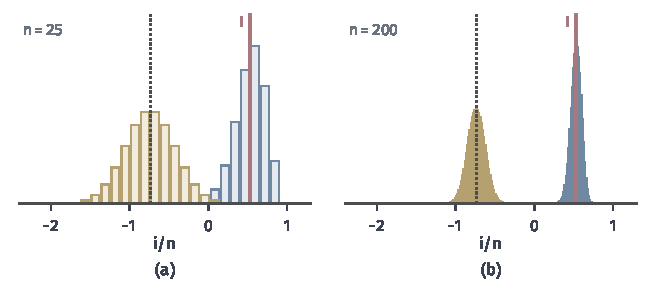
\includegraphics[width=110mm]{figures/07-probability/06-channel-coding/matplotlib/dcc-info-density/figure.pdf}
 \caption{翻转概率$0.1$的二元对称信道、均匀输入时，归一化信息密度$i/n=\frac1n\log_2[W^n(y^n\mid x^n)/p^n(y^n)]$的精确分布。蓝色为码字与其输出块的正确配对，黄色为与输出块独立的码字；红线为$I=0.531$，点线为独立配对的均值$-0.737$。(a) $n=25$；(b) $n=200$。}
 \label{fig:dcc-info-density}
\end{BookInlineFigure}

\paragraph{可达性的证明}

\begin{theorem}[可达性]
\label{thm:dcc-achievability}
对离散无记忆信道，每个$0\leq R<C$都是可达速率。
\end{theorem}

\begin{proof}
$R=0$已知可达，下设$0<R<C$。取最优输入分布$q^{*}$，于是$I(X;Y)=C$；再取$\epsilon>0$使$R<C-3\epsilon$。令$M=\lceil2^{nR}\rceil$，则$M-1<2^{nR}$。

随机码本。独立地抽取$M$个码字$\mathsf{X}^n(1),\dots,\mathsf{X}^n(M)$，每个码字的$n$个符号独立同服从$q^{*}$，即每个码字服从$(q^{*})^n$。码本抽定以后告诉收发双方，传输消息$m$时发送$\mathsf{X}^n(m)$。

解码规则。收到$y^n$后，若恰有一个$\hat{m}$使$(\mathsf{X}^n(\hat{m}),y^n)\in A_{\epsilon}^{(n)}$，就判为$\hat{m}$；否则判为$1$。

错误分析。固定消息$m$，设发送的是$\mathsf{X}^n(m)$，输出为$Y^n$。定义事件
\[
 E_j=\bigl\{(\mathsf{X}^n(j),Y^n)\in A_{\epsilon}^{(n)}\bigr\},\qquad j=1,\dots,M .
\]
若$E_m$发生而其余$E_j$都不发生，解码器判为$m$。所以判错的事件包含于$E_m^{\mathrm{c}}\cup\bigcup_{j\neq m}E_j$，由并集上界，对码本与信道噪声一起取概率，
\[
 \mathbb{E}[\lambda_m]\leq\mathbb{P}(E_m^{\mathrm{c}})+\sum_{j\neq m}\mathbb{P}(E_j) ,
\]
这里$\lambda_m$随码本而变，$\mathbb{E}$是对码本求平均。

第一项：$(\mathsf{X}^n(m),Y^n)$的各对$(X_i,Y_i)$独立同服从$q^{*}(x)W(y\mid x)$，由引理~\ref{lem:dcc-joint-aep}(1)，$\mathbb{P}(E_m^{\mathrm{c}})\to0$。

第二项：$j\neq m$时，$\mathsf{X}^n(j)$与$(\mathsf{X}^n(m),Y^n)$独立，而$Y^n$的边缘分布是$(p^{*})^n$。由式~\eqref{eq:dcc-independent-typical}，$\mathbb{P}(E_j)\leq2^{-n(C-3\epsilon)}$。合起来，
\[
 \mathbb{E}[\lambda_m]\leq\mathbb{P}(E_m^{\mathrm{c}})+(M-1)\,2^{-n(C-3\epsilon)}\leq\mathbb{P}(E_m^{\mathrm{c}})+2^{-n(C-3\epsilon-R)} .
\]
右边与$m$无关，记为$\delta_n$；因为$C-3\epsilon-R>0$，$\delta_n\to0$。

选出确定码本。对$m$取平均，随机码本的平均错误概率满足$\mathbb{E}[P_{\mathrm{e}}]\leq\delta_n$。一个随机变量不可能处处大于它的均值，所以存在某个具体码本，其平均错误概率$P_{\mathrm{e}}^{(n)}\leq\delta_n$。对每个$n$取这样一个码本，得到$M_n=\lceil2^{nR}\rceil\geq2^{nR}$且$P_{\mathrm{e}}^{(n)}\to0$的码列。
\end{proof}

为什么码率低于互信息就够了？错误有两个来源。正确码字不典型，这由大数律控制，与码率无关。某个竞争码字碰巧看起来与输出匹配，每个竞争者的机会约为$2^{-nC}$，竞争者约有$2^{nR}$个，总机会约为$2^{-n(C-R)}$；只要$R<C$，它就按指数趋于零。这正是计数图景的严格版本：小椭圆的个数$2^{nR}$少于能容纳的数目$2^{nC}$。

\paragraph{一个精确的数值}
在翻转概率$0.1$、均匀输入的二元对称信道上，证明中的两项都可以按$k$的二项分布精确求和，不必用指数上界。图~\ref{fig:dcc-random-coding-bound}画出$\mathbb{P}(E_m^{\mathrm{c}})+(M-1)\mathbb{P}(E_j)$随块长的变化（在$1$处截断），容差取$\epsilon=(C-R)/2$。$R=0.25$时，$n=1000$的值约为$4.7\times10^{-6}$，$n=2000$时约为$2.2\times10^{-10}$；$R=0.40$更靠近容量，$n=1000$时仍有$0.031$，$n=2000$时降到$0.0020$。越靠近容量，需要的块长越长。$R=0.60$高于容量，这个上界始终为$1$；下一小节证明这不只是上界的缺陷。

\begin{BookInlineFigure}
 \centering
 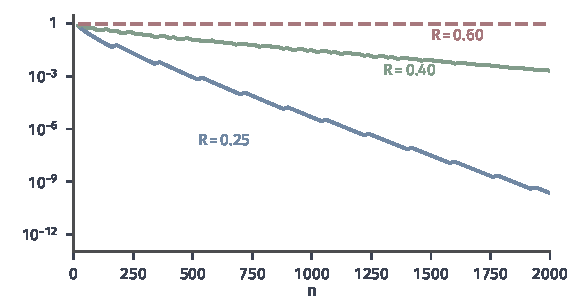
\includegraphics[width=96mm]{figures/07-probability/06-channel-coding/matplotlib/dcc-random-coding-bound/figure.pdf}
 \caption{翻转概率$0.1$的二元对称信道上随机编码的错误上界$\mathbb{P}(E_m^{\mathrm{c}})+(M-1)\mathbb{P}(E_j)$，$M=\lceil2^{nR}\rceil$，均匀输入，两项都按二项分布精确计算，值在$1$处截断，纵轴为对数坐标。蓝线$R=0.25$与绿线$R=0.40$低于容量$0.531$，容差$\epsilon=(C-R)/2$；红色虚线$R=0.60$高于容量，取$\epsilon=0.05$。曲线的小幅锯齿来自$k$的整数取值。}
 \label{fig:dcc-random-coding-bound}
\end{BookInlineFigure}

\paragraph{存在不等于可用}
证明只说明好码本存在，没有给出低成本的编码与解码。随机码本没有结构，必须整体存储$M n$个符号；典型性解码要把输出块与全部$M$个码字逐一比较。$R=0.25$、$n=1000$时，$M=2^{250}$，无论存储还是比较都无法实现。用代数结构降低编码与解码的代价，是第~\ref{chap:channel-codes}章的任务。

\subsection{逆定理}
\label{sec:dcc-converse}

可达性给出了容量以下的速率。反方向要说明：码率高于$C$时，无论码本与解码器如何设计，错误都不能趋于零。思路是把“判对”翻译成“消息与输出之间有很多信息”，再用引理~\ref{lem:dcc-block-bound}说明信息不会超过$nC$。

翻译所用的工具是第~\ref{chap:information-measures}章的Fano不等式。设消息变量取值于$M\geq2$个标签，$\hat{M}$是对它的判决，$P_{\mathrm{e}}=\mathbb{P}(\hat{M}\neq M)$。以比特计，Fano不等式为
\[
 H(M\mid\hat{M})\leq h_2(P_{\mathrm{e}})+P_{\mathrm{e}}\log_2(M-1)\leq1+P_{\mathrm{e}}\log_2M ,
\]
第二步用了$h_2\leq1$。它说判错的机会小，判决后剩余的不确定性就少。

\begin{theorem}[逆定理]
\label{thm:dcc-converse}
设$(M,n)$码用于离散无记忆信道，编码器不使用反馈，$M\geq2$，消息均匀分布。则平均错误概率满足
\begin{equation}
 P_{\mathrm{e}}\geq1-\frac{nC+1}{\log_2M} .
 \label{eq:dcc-fano-bound}
\end{equation}
特别地，若$M\geq2^{nR}$，则$P_{\mathrm{e}}\geq1-C/R-1/(nR)$；当$R>C$时，任何这样的码列都满足
\begin{equation}
 \liminf_{n\to\infty}P_{\mathrm{e}}^{(n)}\geq1-\frac CR>0 ,
 \label{eq:dcc-weak-converse}
\end{equation}
所以$R$不可达。
\end{theorem}

\begin{proof}
消息均匀，$H(M)=\log_2M$。按条件熵与互信息的关系，
\[
 \log_2M=H(M\mid\hat{M})+I(M;\hat{M}) .
\]
第一项用Fano不等式：$H(M\mid\hat{M})\leq1+P_{\mathrm{e}}\log_2M$。

第二项用数据处理不等式两次。判决$\hat{M}=g(Y^n)$只依赖输出块，所以$I(M;\hat{M})\leq I(M;Y^n)$。码字$X^n=f(M)$由消息决定，而且因为没有反馈，给定$X^n$后$Y^n$的条件分布由式~\eqref{eq:dcc-memoryless}决定，不再依赖$M$：$M$、$X^n$、$Y^n$按顺序构成Markov链，于是$I(M;Y^n)\leq I(X^n;Y^n)$。再由引理~\ref{lem:dcc-block-bound}，
\[
 I(M;\hat{M})\leq I(X^n;Y^n)\leq nC .
\]

两项相加，得到
\[
 \log_2M\leq1+P_{\mathrm{e}}\log_2M+nC ,
\]
两边除以$\log_2M$并移项，就是式~\eqref{eq:dcc-fano-bound}。若$\log_2M\geq nR$，则$(nC+1)/\log_2M\leq C/R+1/(nR)$，第二个结论随之成立。
\end{proof}

图~\ref{fig:dcc-fano-bound}画出翻转概率$0.1$的二元对称信道上的下界$1-C/R-1/(nR)$。容量以下它是零，不构成限制；容量以上它为正，并且随$n$增大升向极限$1-C/R$。例如$R=1$（不加任何冗余）时，极限下界是$1-0.531=0.469$。

\begin{BookInlineFigure}
 \centering
 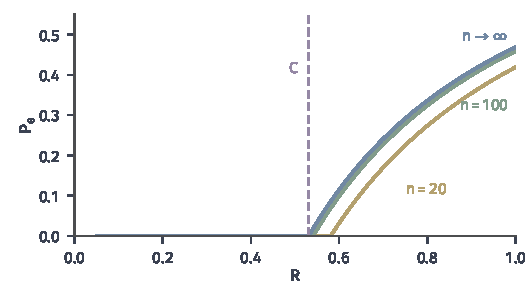
\includegraphics[width=90mm]{figures/07-probability/06-channel-coding/matplotlib/dcc-fano-bound/figure.pdf}
 \caption{翻转概率$0.1$的二元对称信道上，任何$M\geq2^{nR}$的码的平均错误概率下界$1-C/R-1/(nR)$（负值截为零），作为码率$R$的函数：黄线$n=20$，绿线$n=100$，蓝线为$n\to\infty$的极限$1-C/R$；紫色虚线为容量$C=0.531$。}
 \label{fig:dcc-fano-bound}
\end{BookInlineFigure}

证明在两个地方用到了模型假设。数据处理的第二步需要“给定码字后输出与消息无关”，有反馈时编码器的后续输入依赖此前的输出，这一步要重新论证。引理~\ref{lem:dcc-block-bound}需要无记忆。另外，下界$1-C/R$只说错误不能趋于零，并没有说错误趋于$1$。离散无记忆信道上，码率高于容量时错误概率实际上趋于$1$，这称为强逆定理；证明要控制信息密度的集中程度，而不只是它的均值，篇幅较长，可查阅~\scite{math-cover2006information}。

\subsection{最大错误概率}
\label{sec:dcc-max-error}

可达性证明控制的是平均错误概率：大多数消息很少出错，但可能有少数消息出错很多。如果消息不是均匀出现的，例如第~\ref{chap:channel-codes}章把压缩后的索引送进信道时，平均错误小并不能保证实际错误小。需要的是每条消息都可靠，即$\lambda_{\max}$小。

办法是删去坏消息。平均值为$P_{\mathrm{e}}$的一组非负数中，超过平均值两倍的不会多于一半：若超过$2P_{\mathrm{e}}$的有$k\geq1$个，则
\[
 MP_{\mathrm{e}}=\sum_{m}\lambda_m>k\cdot2P_{\mathrm{e}} ,
\]
所以$k<M/2$。这是第~\ref{chap:tail-probabilities}章Markov不等式在均匀分布上的形式。

\begin{lemma}[删去坏码字]
\label{lem:dcc-expurgation}
设$(M,n)$码的平均错误概率为$P_{\mathrm{e}}$，$M\geq2$。则可以从中保留至少$\lceil M/2\rceil$条消息，得到一个最大错误概率不超过$2P_{\mathrm{e}}$的码。
\end{lemma}

\begin{proof}
保留$\lambda_m\leq2P_{\mathrm{e}}$的消息，由上面的计数，保留的个数至少为$\lceil M/2\rceil$。码字不变；解码器把原来判给被删消息的输出块任意改判给一条保留的消息。对保留的消息$m$，判为$m$的输出块只增不减，所以它的条件错误概率不超过原来的$\lambda_m\leq2P_{\mathrm{e}}$。
\end{proof}

这一步称为\term{码字删除}（expurgation）。码率的损失是
\[
 \frac{\log_2M}{n}-\frac{\log_2\lceil M/2\rceil}{n}\leq\frac1n ,
\]
随块长趋于零。所以对$R<C$，先取$R<R'<C$，用可达性得到$M_n\geq2^{nR'}$、平均错误趋于零的码列，再删去一半消息，得到$\lceil M_n/2\rceil\geq2^{nR'-1}\geq2^{nR}$（$n$足够大时）且$\lambda_{\max}\to0$的码列。这就完成了定理~\ref{thm:dcc-coding-theorem}中关于最大错误概率的部分。反方向，最大错误不小于平均错误，逆定理对最大错误口径同样成立。两种口径给出相同的容量。

图~\ref{fig:dcc-expurgation}是一个具体的例子：随机抽取$16$个长度为$14$的二元码字（码率$\tfrac27$），在翻转概率$0.1$的二元对称信道上用最大似然解码（并列时判给编号较小的消息），对全部$2^{14}$个输出块精确求出每条消息的$\lambda_m$。平均错误概率为$0.069$，最差的消息却达到$0.253$。原因是它与另一个码字只差两位，两者似然相同的输出块按并列规则判给了编号较小的那一条，那一条的错误只有$0.040$。删去这一条消息后，剩余$15$条消息的最大错误概率为$0.127$，不超过$2P_{\mathrm{e}}=0.139$，码率变为$\log_215/14\approx0.279$。

\begin{BookInlineFigure}
 \centering
 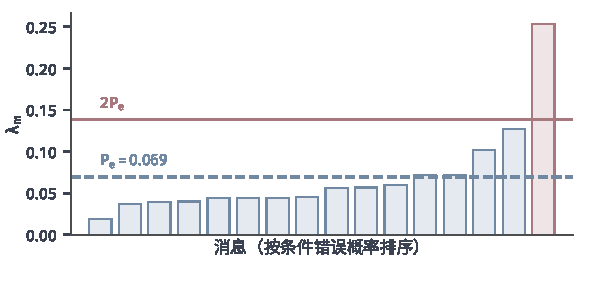
\includegraphics[width=100mm]{figures/07-probability/06-channel-coding/matplotlib/dcc-expurgation/figure.pdf}
 \caption{一个随机二元码（$16$个码字，长度$14$，随机种子$1$）在翻转概率$0.1$的二元对称信道上用最大似然解码时，各消息的条件错误概率$\lambda_m$，按大小排序，均为精确值。蓝色虚线为平均错误概率$0.069$，红线为其两倍；红色柱是被删去的消息。}
 \label{fig:dcc-expurgation}
\end{BookInlineFigure}

删除只在渐近意义下“免费”：$1/n$比特的损失随块长消失，但在有限块长下它是真实的代价。对短码，设计时直接控制每条消息的错误，比事后删除更合适。
